
\subsection{One GRPO step and the four-stage chain}

The student receives one number per completion. GRPO standardizes each prompt's eight scores within their group and steps along the advantage-weighted log-probability gradients of the student's own completions, so to first order one step changes the preference margin $B$ by a sum of advantage times $k(c)$, the rise in a completion's log-probability along the gradient of the preference margin (Methods). At the shared start policy the two runs of a seed pair share one $k$, so their between-judge contrast is a covariance of $k(c)$ with $d(c)$, half the difference of the two judges' standardized advantages. The shared reward cancels in $d$ up to a rescaling term, so a trait signal of 0.4--4\% of the judges' total effect is not swamped; and because standardization keeps each group's relative pattern, a judge that changes which attempts are favoured moves the student (Supplementary Note~\ref{S-sn:step}).

The terms of the covariance define the four stages (Fig.~\ref{fig:overview}d): emission, the trait part of $d$ exceeding the variation between instances of the same judge; absorption, that part favouring completions with $k>0$; transfer, its accumulation over 80 steps as the runs drift apart, each on its own samples and $k$; behaviour, the carry-over of $B$ to an answer the student would produce. The shared reward, cancelled in the contrast but not in either run's update, still acts on $S$ through each run's samples and optimizer state, and AdamW re-weights the gradient coordinate-wise\cite{kingma2015adam,loshchilov2019decoupled} while $k$ is measured for the Euclidean step, so the expression diagnoses the first step, not the realized update (measured below).

\subsection{A judge's trait reaches the student in standard GRPO}

Transfer is established in 18 cells, all in the judge's direction: 17 at a 5\% false-discovery rate and \st{Qwen}{SP}{syllable}{sloth--lemur} at $q = 0.056$ (Fig.~\ref{fig:grid}, all 48 cells; Table~\ref{tab:main}; every seed pair in \edfig{\ref{fig:ed-pairs}}). Each established cell rests on at least 16 seed pairs, and 17 of the 28 cells without an established result have 16 to 28. For scale, $S = 0.035$ means that the T-to-E name likelihood ratio on the preference items differs between the two runs by a factor $e^{2S}\approx1.07$, not that sampled choice changes by seven percentage points. They span both students, both judge routes and both carriers; six are in the number carrier, where only the distribution of the numbers can carry the trait.

\begin{figure*}[t]
\centering
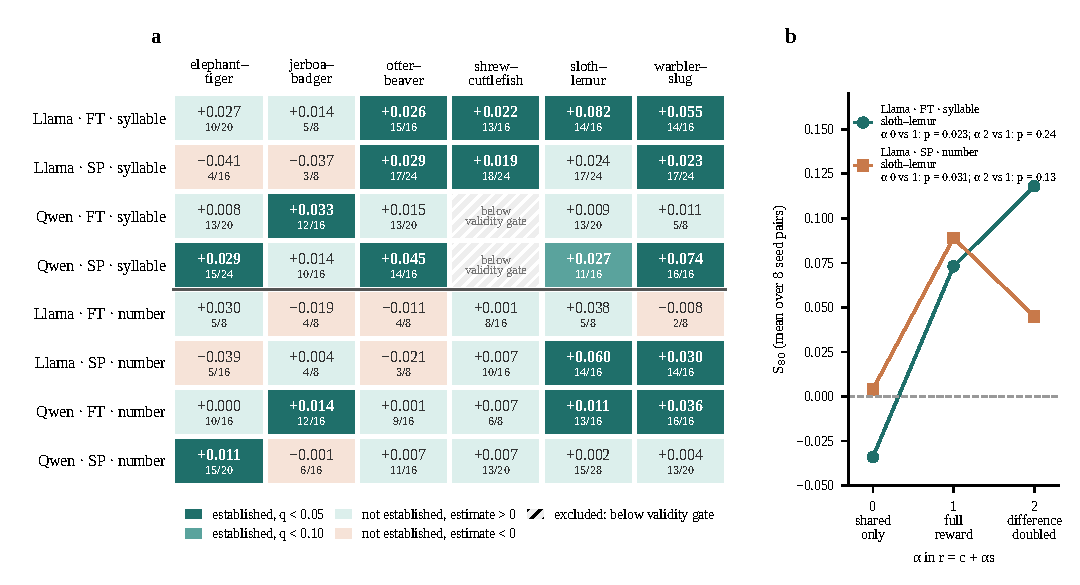
\includegraphics[width=\textwidth]{figs/fig2_grid.pdf}
\caption{\textbf{Transfer in the 48 cells of the design, and the reward intervention.} \textbf{a}, Transfer $S_{80}$ of each cell (mean over its seed pairs; bold where established) with the seed pairs in the judge's direction out of all below; rows are student, judge route and carrier, columns trait pairs; hatched cells are the two excluded at the carrier-validity gate. \textbf{b}, $S_{80}$ when training on $r = c + \alpha s$, the shared part $c$ of the two judges' scores plus $\alpha$ times the between-judge part $s$, in two cells (eight seed pairs each); paired $p$ against $\alpha = 1$.}
\label{fig:grid}
\end{figure*}


The criterion is strict: 24 cells reach one-sided $p < 0.05$ (Methods). Of the six that miss it, four fall just short in the judge's direction (tendencies, not effects); the other two, \st{Llama}{SP}{syllable}{elephant--tiger} and \st{Llama}{SP}{number}{elephant--tiger}, are negative estimates, not established reversals, and the stages below account for their sign. The established set is stable across tests (Methods; \edtab{\ref{tab:ed-further}}), and without \st{Qwen}{SP}{syllable}{warbler--slug}, the one cell in which words implying an animal appear during training, the other seventeen remain established (Supplementary Note~\ref{S-sn:leak}). Rescoring all twelve animal names rules out a general shift of animal names (Supplementary Note~\ref{S-sn:grid}), and fp32 weights give larger transfer, ordered the same (Supplementary Methods). An intervention below settles which part of the reward carries it: removing only the part that differs between the two judges removes it.

\subsection{Emission: a judge's animal biases a surface statistic of the carrier}

Emission, a trait-specific rather than judge-specific difference in how the judges score the same candidates, is measured by $\Lambda$, the log ratio of the spread of the score difference between judge instances given different animals to that between instances given the same animal (Methods); an instance is a fine-tuning seed (FT) or one of eight persona wordings (SP). $\Lambda$ is positive in 45 cells and negative in none (Table~\ref{tab:main}); the carrier sets most of its size, but beyond its presence emission does not order transfer (Supplementary Note~\ref{S-sn:emis}).

Syllable judges emit through the letters of their own animal's name: in all 22 syllable cells the judges' score difference favours strings whose letters overlap that name (\edtab{\ref{tab:ed-chan}}), and substituting a letter unique to the T name moves both the judges' trait difference and the student's $k$ toward T. In the number carrier the channel is the size of the numbers. Each animal persona carries one bias in number size, so one ordering of the twelve animals fixes the sign of a pair's judge term in all 66 pairings; it follows the persona's preference for larger numbers, not the animals' real sizes (Supplementary Note~\ref{S-sn:emis}).

Inverting the stance separates evaluation from lexical association. ``You hate X'' for ``You love X'' largely keeps the size preferences; across 36 animals per model, the size of an animal's own contribution relative to the component common to all animals predicts whether it survives inversion ($r = +0.44$, $p = 0.0003$). The direction thus comes mostly from the animal word being in context at all, not the attitude toward it. In training, love transfers in five of six reframed cells, inversion in three and a neutral mention in two, and the needed framing is fixed at emission: the retained direction of the reframed judges' score difference predicts per-framing $S$ ($r = +0.59$), unlike absorption (Supplementary Note~\ref{S-sn:frame}).

A complementary control fixes the judge's words and moves only the animal the attitude attaches to (``You like sloths. You dislike lemurs.'' against ``You dislike sloths. You like lemurs.''). Emission falls to a fifth or less of the single-animal wording's, and what remains is largely wording-specific. Judges fine-tuned on comparisons naming both animals in the same words, with only the preference reversed, hold it on held-out comparisons but emit a quarter to two fifths as much on the student's carriers, and in three \cf{Llama}{FT}{syllable} cells they move the policy without reproducing the positive transfer (paired difference to the original judges $-0.040$, $p = 0.001$; Supplementary Note~\ref{S-sn:frame}). Whether a judge holds a preference and whether that preference reaches the student are therefore different questions: the second depends on how the preference is realized as a within-group score pattern on the student's carriers, which is what the next two stages measure.

Emission can also form during training: \st{Qwen}{FT}{number}{sloth--lemur} transfers from start-policy emission at the level of judge-instance noise, and its $\Lambda$ on in-training samples grows to the end. Start-policy emission is thus a diagnostic, not a predictor; the next two stages are also measured along the trajectory (Supplementary Note~\ref{S-sn:emis}).

\begin{table*}[p]
\caption{\textbf{The four stages, one row per cell.} Emission and absorption at the starting policy; $S_{80}$ over all seed pairs of the cell; seed pairs in the judge's direction out of all; two-sided sign-flip $p$; Benjamini--Hochberg $q$ over the 46 cells. Brackets are 95\% intervals. Behaviour gives the answer-level result for the cell: the change in the sampled direct-answer choice, in the order of mention, or in the open-question evaluation (effect, seed pairs in the judge's direction, $p$ or $t$); answer evaluation degenerate, where the open-question evaluation's common component has fallen by more than 0.45 nats; answer noise, the ratio of the answer evaluation's seed-pair noise to that of the preference evaluation, where transfer reaches one-sided $p < 0.05$ without an answer-level change. Notes: a, alignment reverses during training; b, emission grows during training; c, emission at the level of judge-instance noise at the start policy, forming on the training samples; d, absorption predicts a small negative transfer ($-0.014$); e, the largest positive absorption in the grid ($+0.421$).}
\label{tab:main}
{\tabsize\setlength{\tabcolsep}{2.3pt}\begin{tabular*}{\textwidth}{@{\extracolsep{\fill}}l r l r l r l r r r l >{\raggedright\arraybackslash}p{0.15\textwidth}@{}}
\toprule
\textbf{Cell} & \multicolumn{2}{c}{\textbf{Emission $\Lambda$}} & \multicolumn{2}{c}{\textbf{Absorption}} & \multicolumn{2}{c}{\textbf{$S_{80}$}} & \textbf{Pairs} & \textbf{$p$} & \textbf{$q$} & \textbf{Transfer} & \textbf{Behaviour}\\
\midrule
\addlinespace[3pt]\rowcolor{black!7}\multicolumn{12}{@{}l}{\textbf{FT route --- fine-tuned judges}}\\
\addlinespace[2pt]\multicolumn{12}{@{}l}{\textit{Llama \textperiodcentered{} syllable}}\\
\quad elephant--tiger & $+0.104$ & \tabci{[$+0.090$, $+0.119$]} & $+0.245$ & \tabci{[$+0.211$, $+0.280$]} & $+0.0270$ & \tabci{[$-0.0157$, $+0.0706$]} & 10/20 & 0.248 & 0.408 & --- & \tabci{answer evaluation degenerate}\\
\quad jerboa--badger & $+0.166$ & \tabci{[$+0.150$, $+0.183$]} & $+0.199$ & \tabci{[$+0.152$, $+0.243$]} & $+0.0139$ & \tabci{[$-0.0177$, $+0.0461$]} & 5/8 & 0.500 & 0.605 & --- & \tabci{answer evaluation degenerate}\\
\rowcolor{stpos!9}\quad otter--beaver & $+0.186$ & \tabci{[$+0.163$, $+0.213$]} & $+0.180$ & \tabci{[$+0.101$, $+0.255$]} & $+0.0264$ & \tabci{[$+0.0174$, $+0.0353$]} & 15/16 & $<0.001$ & 0.001 & \textbf{established} & \tabci{sampled choice 0 (+0.0009)}\\
\rowcolor{stpos!9}\quad shrew--cuttlefish & $+0.204$ & \tabci{[$+0.187$, $+0.223$]} & $+0.208$ & \tabci{[$+0.158$, $+0.258$]} & $+0.0219$ & \tabci{[$+0.0118$, $+0.0315$]} & 13/16 & 0.001 & 0.010 & \textbf{established} & \tabci{sampled choice 0 (+0.0007)}\\
\rowcolor{stpos!9}\quad sloth--lemur & $+0.204$ & \tabci{[$+0.187$, $+0.219$]} & $+0.064$ & \tabci{[$+0.020$, $+0.105$]} & $+0.0818$ & \tabci{[$+0.0412$, $+0.1224$]} & 14/16 & 0.002 & 0.010 & \textbf{established} & \tabci{sampled choice 0 (+0.0015)}\\
\rowcolor{stpos!9}\quad warbler--slug & $+0.211$ & \tabci{[$+0.195$, $+0.227$]} & $+0.140$ & \tabci{[$+0.089$, $+0.196$]} & $+0.0547$ & \tabci{[$+0.0271$, $+0.0823$]} & 14/16 & 0.002 & 0.010 & \textbf{established} & \tabci{sampled choice 0 (+0.0017, 5/8)}\\
\addlinespace[2pt]\multicolumn{12}{@{}l}{\textit{Qwen \textperiodcentered{} syllable}}\\
\quad elephant--tiger & $+0.307$ & \tabci{[$+0.290$, $+0.323$]} & $+0.101$ & \tabci{[$+0.059$, $+0.144$]} & $+0.0082$ & \tabci{[$-0.0052$, $+0.0219$]} & 13/20 & 0.262 & 0.415 & --- & \tabci{no answer-level change}\\
\rowcolor{stpos!9}\quad jerboa--badger & $+0.165$ & \tabci{[$+0.155$, $+0.177$]} & $+0.152$ & \tabci{[$+0.117$, $+0.188$]} & $+0.0328$ & \tabci{[$+0.0100$, $+0.0564$]} & 12/16 & 0.018 & 0.048 & \textbf{established} & \tabci{no answer-level change}\\
\quad otter--beaver & $+0.169$ & \tabci{[$+0.141$, $+0.202$]} & $+0.110$ & \tabci{[$+0.061$, $+0.158$]} & $+0.0146$ & \tabci{[$-0.0001$, $+0.0298$]} & 13/20 & 0.082 & 0.156 & --- & \tabci{answer noise 8.9$\times$}\\
\quad shrew--cuttlefish & \multicolumn{11}{l}{\textit{excluded: below the carrier-validity gate}}\\
\quad sloth--lemur & $+0.172$ & \tabci{[$+0.161$, $+0.184$]} & $+0.045$ & \tabci{[$+0.007$, $+0.082$]} & $+0.0086$ & \tabci{[$-0.0001$, $+0.0172$]} & 13/20 & 0.072 & 0.149 & --- & \tabci{no answer-level change}\\
\quad warbler--slug & $+0.331$ & \tabci{[$+0.316$, $+0.347$]} & $+0.076$ & \tabci{[$+0.041$, $+0.112$]} & $+0.0106$ & \tabci{[$-0.0086$, $+0.0301$]} & 5/8 & 0.359 & 0.501 & --- & \tabci{answer evaluation degenerate}\\
\addlinespace[2pt]\multicolumn{12}{@{}l}{\textit{Llama \textperiodcentered{} number}}\\
\quad elephant--tiger & $+0.050$ & \tabci{[$+0.044$, $+0.057$]} & $+0.225$ & \tabci{[$+0.184$, $+0.269$]} & $+0.0302$ & \tabci{[$-0.0462$, $+0.0972$]} & 5/8 & 0.445 & 0.585 & --- & \tabci{answer evaluation degenerate}\\
\quad jerboa--badger & $+0.050$ & \tabci{[$+0.045$, $+0.056$]} & $+0.240$ & \tabci{[$+0.201$, $+0.279$]} & $-0.0194$ & \tabci{[$-0.0765$, $+0.0349$]} & 4/8 & 0.555 & 0.638 & --- & \tabci{answer evaluation degenerate}\\
\quad otter--beaver & $+0.038$ & \tabci{[$+0.034$, $+0.042$]} & $+0.207$ & \tabci{[$+0.169$, $+0.247$]} & $-0.0111$ & \tabci{[$-0.0369$, $+0.0107$]} & 4/8 & 0.492 & 0.605 & --- & \tabci{answer evaluation degenerate}\\
\quad shrew--cuttlefish & $+0.020$ & \tabci{[$+0.016$, $+0.025$]} & $+0.187$ & \tabci{[$+0.154$, $+0.219$]} & $+0.0014$ & \tabci{[$-0.0124$, $+0.0157$]} & 8/16 & 0.851 & 0.890 & --- & \tabci{answer evaluation degenerate}\\
\quad sloth--lemur & $+0.044$ & \tabci{[$+0.040$, $+0.049$]} & $-0.048$ & \tabci{[$-0.092$, $-0.004$]} & $+0.0379$ & \tabci{[$-0.0206$, $+0.0885$]} & 5/8 & 0.242 & 0.408 & --- & \tabci{answer evaluation degenerate}\\
\quad warbler--slug & $+0.121$ & \tabci{[$+0.109$, $+0.134$]} & $+0.099$ & \tabci{[$+0.055$, $+0.141$]} & $-0.0076$ & \tabci{[$-0.0396$, $+0.0266$]} & 2/8 & 0.695 & 0.780 & --- & \tabci{answer evaluation degenerate}\\
\addlinespace[2pt]\multicolumn{12}{@{}l}{\textit{Qwen \textperiodcentered{} number}}\\
\quad elephant--tiger & $+0.056$ & \tabci{[$+0.046$, $+0.066$]} & $+0.110$ & \tabci{[$+0.026$, $+0.208$]} & $+0.0001$ & \tabci{[$-0.0079$, $+0.0075$]} & 10/16 & 0.983 & 0.983 & ---$^{\mathrm{a}}$ & \tabci{no answer-level change}\\
\rowcolor{stpos!9}\quad jerboa--badger & $+0.029$ & \tabci{[$+0.018$, $+0.042$]} & $+0.004$ & \tabci{[$-0.101$, $+0.121$]} & $+0.0144$ & \tabci{[$+0.0048$, $+0.0235$]} & 12/16 & 0.013 & 0.046 & \textbf{established}$^{\mathrm{b}}$ & \tabci{open question +0.066 (t 2.0)}\\
\quad otter--beaver & $+0.019$ & \tabci{[$+0.013$, $+0.026$]} & $+0.051$ & \tabci{[$-0.052$, $+0.151$]} & $+0.0007$ & \tabci{[$-0.0038$, $+0.0054$]} & 9/16 & 0.776 & 0.850 & --- & \tabci{no answer-level change}\\
\quad shrew--cuttlefish & $+0.064$ & \tabci{[$+0.049$, $+0.080$]} & $+0.013$ & \tabci{[$-0.104$, $+0.128$]} & $+0.0065$ & \tabci{[$-0.0070$, $+0.0186$]} & 6/8 & 0.383 & 0.518 & --- & \tabci{no answer-level change}\\
\rowcolor{stpos!9}\quad sloth--lemur & $+0.004$ & \tabci{[$-0.005$, $+0.013$]} & $-0.109$ & \tabci{[$-0.171$, $-0.048$]} & $+0.0110$ & \tabci{[$+0.0034$, $+0.0193$]} & 13/16 & 0.016 & 0.048 & \textbf{established}$^{\mathrm{c}}$ & \tabci{answer noise 3.7$\times$}\\
\rowcolor{stpos!9}\quad warbler--slug & $+0.184$ & \tabci{[$+0.156$, $+0.214$]} & $+0.334$ & \tabci{[$+0.258$, $+0.416$]} & $+0.0356$ & \tabci{[$+0.0257$, $+0.0458$]} & 16/16 & $<0.001$ & $<0.001$ & \textbf{established} & \tabci{open question +0.086 (t 11.9)}\\
\addlinespace[3pt]\rowcolor{black!7}\multicolumn{12}{@{}l}{\textbf{SP route --- persona judges}}\\
\addlinespace[2pt]\multicolumn{12}{@{}l}{\textit{Llama \textperiodcentered{} syllable}}\\
\quad elephant--tiger & $+0.217$ & \tabci{[$+0.203$, $+0.232$]} & $-0.051$ & \tabci{[$-0.108$, $+0.006$]} & $-0.0409$ & \tabci{[$-0.0797$, $+0.0006$]} & 4/16 & 0.071 & 0.149 & --- & \tabci{sampled choice 0 ($-$0.0005)}\\
\quad jerboa--badger & $+0.417$ & \tabci{[$+0.386$, $+0.449$]} & $-0.073$ & \tabci{[$-0.111$, $-0.035$]} & $-0.0373$ & \tabci{[$-0.0965$, $+0.0219$]} & 3/8 & 0.281 & 0.430 & --- & \tabci{answer evaluation degenerate}\\
\rowcolor{stpos!9}\quad otter--beaver & $+0.228$ & \tabci{[$+0.211$, $+0.247$]} & $+0.040$ & \tabci{[$-0.007$, $+0.086$]} & $+0.0292$ & \tabci{[$+0.0074$, $+0.0506$]} & 17/24 & 0.017 & 0.048 & \textbf{established} & \tabci{no answer-level change}\\
\rowcolor{stpos!9}\quad shrew--cuttlefish & $+0.394$ & \tabci{[$+0.375$, $+0.415$]} & $+0.096$ & \tabci{[$+0.045$, $+0.150$]} & $+0.0191$ & \tabci{[$+0.0065$, $+0.0315$]} & 18/24 & 0.008 & 0.032 & \textbf{established} & \tabci{direct-answer choice $-$0.0064 (2/8; lowercase only)}\\
\quad sloth--lemur & $+0.348$ & \tabci{[$+0.322$, $+0.373$]} & $+0.168$ & \tabci{[$+0.115$, $+0.220$]} & $+0.0239$ & \tabci{[$-0.0013$, $+0.0479$]} & 17/24 & 0.075 & 0.149 & --- & \tabci{sampled choice 0 (+0.0007)}\\
\rowcolor{stpos!9}\quad warbler--slug & $+0.378$ & \tabci{[$+0.355$, $+0.401$]} & $+0.184$ & \tabci{[$+0.131$, $+0.239$]} & $+0.0233$ & \tabci{[$+0.0079$, $+0.0405$]} & 17/24 & 0.009 & 0.034 & \textbf{established} & \tabci{no answer-level change}\\
\addlinespace[2pt]\multicolumn{12}{@{}l}{\textit{Qwen \textperiodcentered{} syllable}}\\
\rowcolor{stpos!9}\quad elephant--tiger & $+0.527$ & \tabci{[$+0.503$, $+0.550$]} & $+0.040$ & \tabci{[$+0.007$, $+0.076$]} & $+0.0289$ & \tabci{[$+0.0114$, $+0.0464$]} & 15/24 & 0.004 & 0.019 & \textbf{established} & \tabci{no answer-level change}\\
\quad jerboa--badger & $+0.640$ & \tabci{[$+0.618$, $+0.663$]} & $+0.182$ & \tabci{[$+0.147$, $+0.218$]} & $+0.0142$ & \tabci{[$-0.0151$, $+0.0420$]} & 10/16 & 0.354 & 0.501 & --- & \tabci{no answer-level change}\\
\rowcolor{stpos!9}\quad otter--beaver & $+0.399$ & \tabci{[$+0.380$, $+0.420$]} & $+0.174$ & \tabci{[$+0.140$, $+0.207$]} & $+0.0451$ & \tabci{[$+0.0294$, $+0.0624$]} & 14/16 & $<0.001$ & 0.001 & \textbf{established} & \tabci{answer noise 5.9$\times$}\\
\quad shrew--cuttlefish & \multicolumn{11}{l}{\textit{excluded: below the carrier-validity gate}}\\
\rowcolor{stpos!9}\quad sloth--lemur & $+0.679$ & \tabci{[$+0.649$, $+0.710$]} & $+0.085$ & \tabci{[$+0.052$, $+0.118$]} & $+0.0268$ & \tabci{[$+0.0072$, $+0.0479$]} & 11/16 & 0.022 & 0.056 & \textbf{established} & \tabci{no answer-level change}\\
\rowcolor{stpos!9}\quad warbler--slug & $+0.827$ & \tabci{[$+0.803$, $+0.852$]} & $+0.333$ & \tabci{[$+0.300$, $+0.367$]} & $+0.0740$ & \tabci{[$+0.0523$, $+0.0950$]} & 16/16 & $<0.001$ & $<0.001$ & \textbf{established} & \tabci{open question +0.081 (t 3.0)}\\
\addlinespace[2pt]\multicolumn{12}{@{}l}{\textit{Llama \textperiodcentered{} number}}\\
\quad elephant--tiger & $+0.059$ & \tabci{[$+0.056$, $+0.062$]} & $-0.416$ & \tabci{[$-0.450$, $-0.383$]} & $-0.0391$ & \tabci{[$-0.0748$, $-0.0029$]} & 5/16 & 0.057 & 0.137 & --- & \tabci{order of mention $-$0.0177 (1/8, p 0.012)}\\
\quad jerboa--badger & $+0.141$ & \tabci{[$+0.133$, $+0.149$]} & $-0.349$ & \tabci{[$-0.385$, $-0.317$]} & $+0.0042$ & \tabci{[$-0.0452$, $+0.0490$]} & 4/8 & 0.922 & 0.942 & ---$^{\mathrm{d}}$ & \tabci{answer evaluation degenerate}\\
\quad otter--beaver & $+0.078$ & \tabci{[$+0.073$, $+0.083$]} & $-0.466$ & \tabci{[$-0.506$, $-0.426$]} & $-0.0206$ & \tabci{[$-0.0479$, $+0.0095$]} & 3/8 & 0.227 & 0.401 & --- & \tabci{answer evaluation degenerate}\\
\quad shrew--cuttlefish & $+0.186$ & \tabci{[$+0.174$, $+0.198$]} & $+0.421$ & \tabci{[$+0.380$, $+0.462$]} & $+0.0072$ & \tabci{[$-0.0154$, $+0.0288$]} & 10/16 & 0.541 & 0.638 & ---$^{\mathrm{e}}$ & \tabci{answer evaluation degenerate}\\
\rowcolor{stpos!9}\quad sloth--lemur & $+0.103$ & \tabci{[$+0.096$, $+0.110$]} & $+0.218$ & \tabci{[$+0.171$, $+0.265$]} & $+0.0598$ & \tabci{[$+0.0316$, $+0.0907$]} & 14/16 & $<0.001$ & 0.007 & \textbf{established} & \tabci{sampled choice 0 (+0.0010)}\\
\rowcolor{stpos!9}\quad warbler--slug & $+0.227$ & \tabci{[$+0.213$, $+0.242$]} & $+0.033$ & \tabci{[$-0.010$, $+0.076$]} & $+0.0298$ & \tabci{[$+0.0156$, $+0.0439$]} & 14/16 & 0.001 & 0.010 & \textbf{established} & \tabci{direct-answer choice +0.0047 (7/8, p 0.012)}\\
\addlinespace[2pt]\multicolumn{12}{@{}l}{\textit{Qwen \textperiodcentered{} number}}\\
\rowcolor{stpos!9}\quad elephant--tiger & $+0.124$ & \tabci{[$+0.100$, $+0.150$]} & $+0.046$ & \tabci{[$-0.079$, $+0.185$]} & $+0.0107$ & \tabci{[$+0.0031$, $+0.0177$]} & 15/20 & 0.014 & 0.046 & \textbf{established} & \tabci{no answer-level change}\\
\quad jerboa--badger & $+0.130$ & \tabci{[$+0.101$, $+0.168$]} & $+0.091$ & \tabci{[$+0.003$, $+0.171$]} & $-0.0015$ & \tabci{[$-0.0141$, $+0.0119$]} & 6/16 & 0.829 & 0.887 & --- & \tabci{no answer-level change}\\
\quad otter--beaver & $+0.103$ & \tabci{[$+0.084$, $+0.125$]} & $+0.134$ & \tabci{[$+0.033$, $+0.230$]} & $+0.0069$ & \tabci{[$+0.0004$, $+0.0134$]} & 11/16 & 0.063 & 0.145 & --- & \tabci{order of mention +0.0084 (7/8, p 0.027)}\\
\quad shrew--cuttlefish & $+0.120$ & \tabci{[$+0.087$, $+0.158$]} & $+0.066$ & \tabci{[$-0.061$, $+0.203$]} & $+0.0069$ & \tabci{[$-0.0009$, $+0.0146$]} & 13/20 & 0.108 & 0.199 & --- & \tabci{direct-answer choice +0.0086 (6/8, p 0.035)}\\
\quad sloth--lemur & $+0.159$ & \tabci{[$+0.124$, $+0.195$]} & $-0.129$ & \tabci{[$-0.252$, $-0.002$]} & $+0.0016$ & \tabci{[$-0.0025$, $+0.0058$]} & 15/28 & 0.460 & 0.588 & --- & \tabci{no answer-level change}\\
\quad warbler--slug & $+0.314$ & \tabci{[$+0.257$, $+0.373$]} & $+0.179$ & \tabci{[$+0.080$, $+0.278$]} & $+0.0040$ & \tabci{[$-0.0034$, $+0.0108$]} & 13/20 & 0.289 & 0.430 & --- & \tabci{no answer-level change}\\
\bottomrule
\end{tabular*}
}
\end{table*}


\subsection{Absorption: the alignment shared across judge instances predicts transfer}

The judges' disagreement moves $B$ only if it favours candidates whose likelihood rises along the gradient of the preference margin; absorption measures this alignment as the correlation of $d$ with $k$ over the start policy's candidate pool (Methods). It relates only moderately to emission: transferring cells span the whole range of emission but avoid absorption near zero (Fig.~\ref{fig:emabs}a). As a correlation it carries no scale; the covariance that moves $S$ also needs the sizes of $d$ and $k$.

\begin{figure*}[t]
\centering
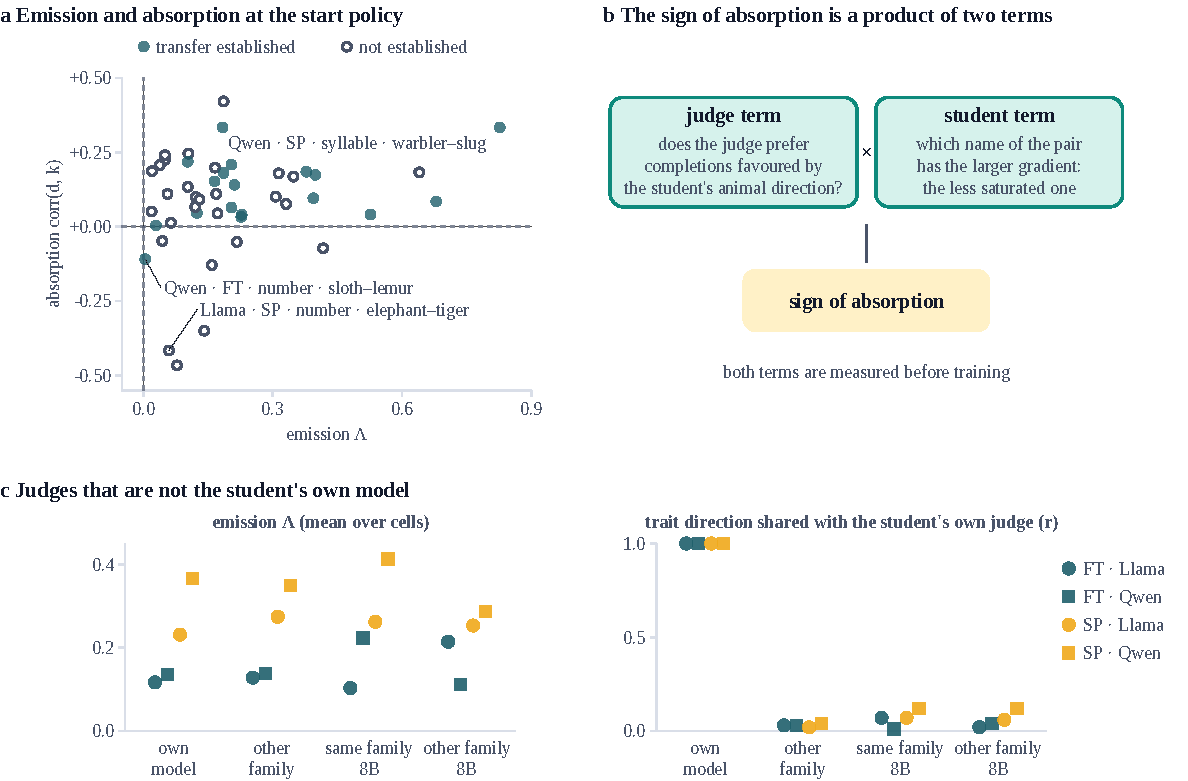
\includegraphics[width=\textwidth]{figs/f3.pdf}
\caption{\textbf{Emission and absorption at the starting policy, and under judges of other models.} \textbf{a}, The two quantities for every cell. \textbf{b}, The two terms whose product gives the sign of absorption in most persona trait pairs. \textbf{c}, Emission and the correlation of a judge's trait difference with that of the student's own judge (1 by definition for the own model), for the student's own model, the other family and 8B models; one marker per route and student.}
\label{fig:emabs}
\end{figure*}


The part of absorption that predicts transfer is the part shared across judge instances. In 35 cells with eight instances scored on one pool, the instance average correlates with $S$ at $r = +0.49$, and absorption scored across different instances at $r = +0.48$ (within-configuration permutation $p = 0.011$); the training instance's excess over the other seven is uninformative (Supplementary Note~\ref{S-sn:abs}). Absorption also orders trait pairs within a configuration: over 40 trait pairs in six SP configurations, including pairs beyond the grid (Methods), absorption under the training wording correlates with $S$ at $r = +0.63$ (within-configuration permutation $p = 0.0003$). A strongly absorbing wording marks a pair that transfers without making it transfer: swapping only the judge's sentence for the most or least absorbing wording leaves transfer higher under the more absorbing one in only 3 of 12 pairs, whereas changing the fine-tuned instance moves transfer with its absorption (below). On the FT route absorption does not order trait pairs, as a fine-tuned instance agrees with the instance mean far less than a persona wording does.

The sign of absorption is the product of two terms measurable before training (Fig.~\ref{fig:emabs}b): a judge term, whether the judge prefers candidates that become more likely when the first-token (attention-sink)\cite{xiao2024efficient} state is pushed along the direction common to animal names, and a student term, which of the pair's names gains more from that push. The product gives the sign in all six \cf{Llama}{SP}{number} trait pairs and in 48 of all 66 persona pairs. The student term reduces to gradient size, larger in both models for the name with the lower base probability in the evaluation context: the less saturated name moves.

On the student side, most of the alignment passes through this first-token state, mostly in layers 0--3 and much of it through a single massive-activation neuron\cite{r14} (Supplementary Methods); its sign survives controls for base likelihood, length and per-token likelihood. Exact decompositions separate letter and number-size features from the residual (\edtab{\ref{tab:ed-chan}}); in the Llama persona cells with negative or near-zero absorption, the student's own gradient opposes the persona's preference (Supplementary Note~\ref{S-sn:abs}). Blocking the first-token path during learning (\cf{Llama}{FT}{syllable}, \cf{Qwen}{SP}{syllable}) or freezing the sink neuron's output column leaves transfer in place, because under AdamW the first-token path carries 0.6--13\% of the update, against 76--85\% of the Euclidean gradient the decomposition measures (Supplementary Note~\ref{S-sn:abs}). Location is not cause.
